%%this is ci2014/book/local_topology.tex
\subsection{Dataset Abstractions}
Visualization tools often decompose data into structure and
attributes~\cite{vtk}. Due to the discrete nature of digital
computers, any continuous function to be estimated must be sampled and
measured at a discrete set of points. However, rendering a
visualization typically requires knowledge of the values between the
samples to produce a perceptually continuous images from arbitrary
viewpoints. Structure encapsulates both the locations and connectivity
relations onto which attributes are superimposed where connectivity
serves to constrain the interpolation problem. Note that some authors
further decompose structure further into topology and
geometry~\cite{weiler}, however, in the context of this research,
topology is synonymous with the structure
abstraction. Figure~\ref{fig:data_hierarchy} outlines the data model
abstraction adopted by \sciwms{}. A dataset is composed of attributes
and an associated structure, further classified as a regular or
irregular topology.

\begin{figure}[ht!]
  \centering
  \begin{subfigure}[t]{0.45\textwidth}
    \includegraphics[width=\textwidth]{../figs/data_model_hierarchy}
  \caption{}
  \label{fig:data_hierarchy}
  \end{subfigure}
  \begin{subfigure}[t]{0.45\textwidth}
    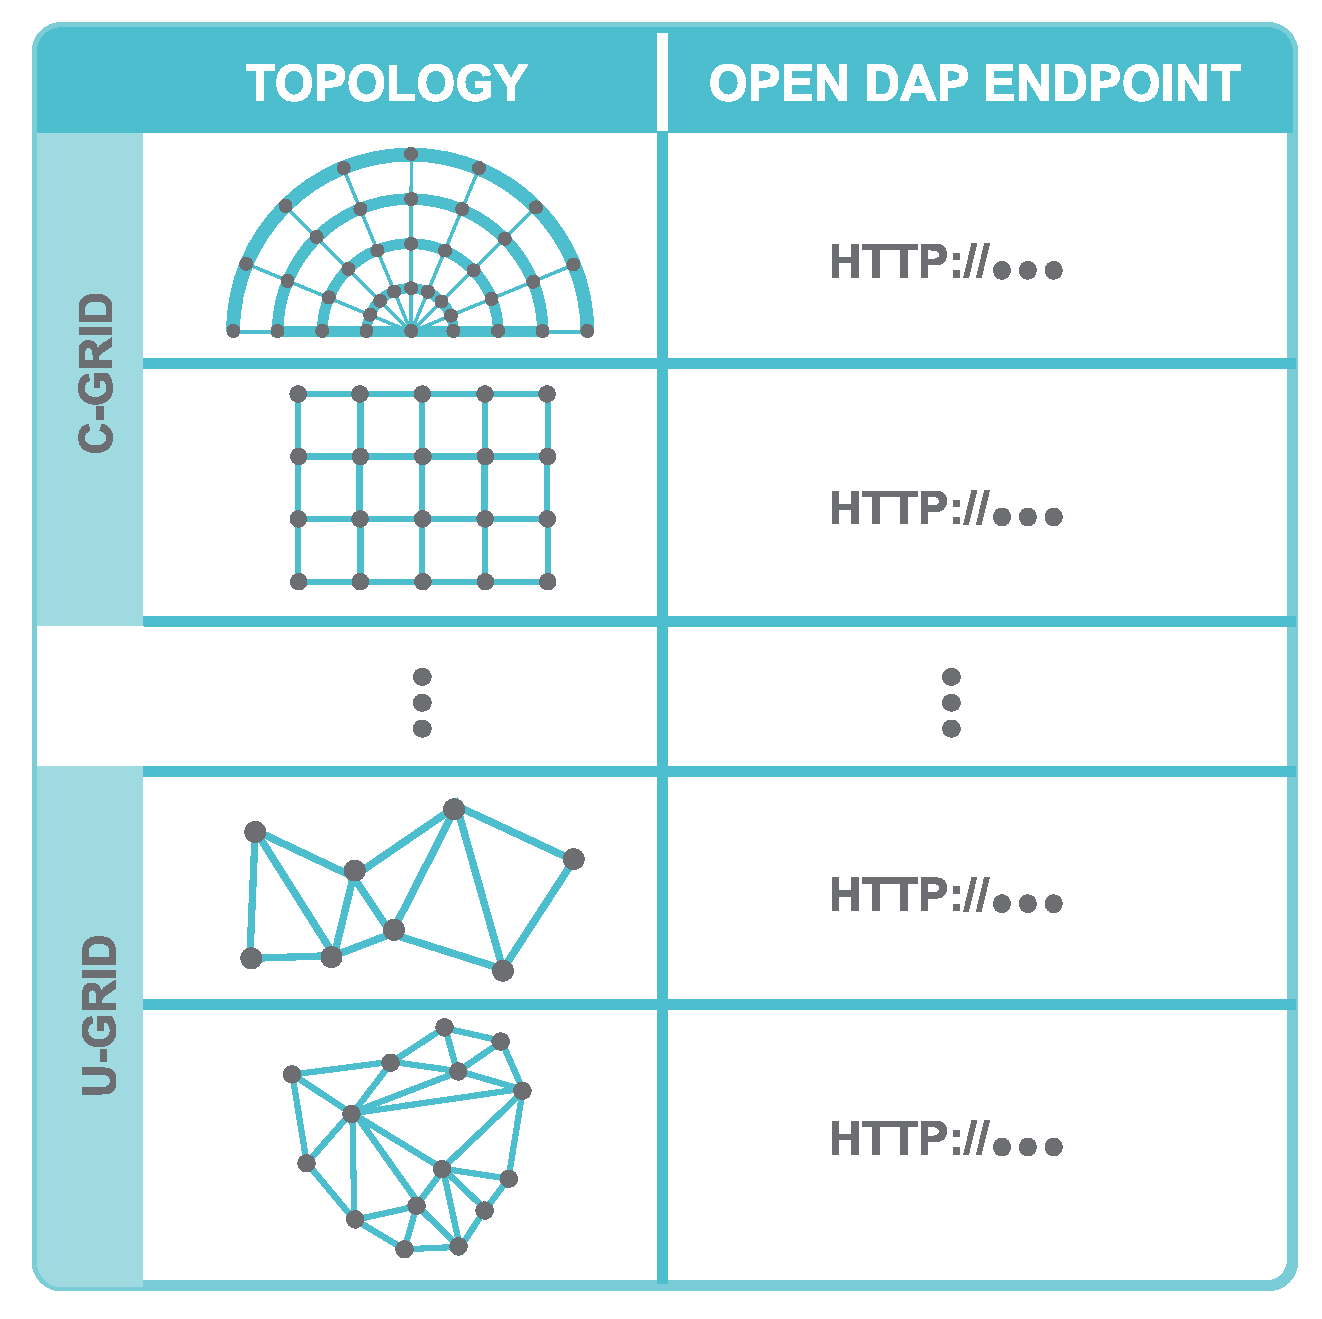
\includegraphics[height=2in]{../figs/sciwms_book_db_topology_endpoint_chart}
    \caption{}
    \label{fig:sciwms_topology_endpoints}
  \end{subfigure}
  \caption{(a) Decomposition hierarchy of the data model. A dataset
    submitted to \sciwms{} is decomposed into attributes and structure
    which is further classified as a regular (\cgrid{}) or irregular
    (\ugrid{}) topologies. (b) \Sciwms{} topology and endpoint data
    store. Topolgies are stored locally in implicit form for \cgrid{}
    or binary R-Tree databases for \ugrid{} topologies. }
\end{figure}

\subsection{Local Topology Cache}

\sciwms{} adopts the \cfugrid{} conventions for implementing the data
model. A topology is always embedded in either $\mathbb{R}^1$,
$\mathbb{R}^2$ or, $\mathbb{R}^3$ where the dimension of a topology
summarizes the connectivity of coordinate locations within the ambient
space. For example, a topology with dimension 0 is a set of
disconnected points, a 1D topology consists of lines or curved
boundaries, a 2D topology is a set of planes or surfaces enclosed by a
set of edges (e.g. triangulation) and a 3D topology specifies a volume
enclosed by a set of faces.

Attributes are defined as numerical quantities that are associated
with the topology. For example, an atmospheric model may estimate wind
direction at the vertices of a triangulated 2D topology or may specify
air temperature at the centroid of cell volumes specified by a 3D
topology. Additionally, attributes maintain their own
dimensionallity. An attribute specifying temperature or
sea-surface-height for example, are scalars while wind directions are
vector valued and tensor valued attributes are also possible.

\subsection{Topology Types}
Topologies are further classified as either regular or irregular ({\bf
  \cgrid{}} and {\bf \ugrid} in \sciwms{} terminology) which admit
different data structures and algorithms for storage and processing.

{\bf \cgrid{}} topologies refer geo-referenced locations and geometries that can be analytically specified, e.g., rectilinear
or curvilinear grids. Storing \cgrid{} topologies amount to storing
the closed form formula. Algorithms for processing \cgrid{}s such as
finding nearest neighbors or finding points that fall withing a
polygonal subset are computed directly using the implicit \cgrid{}
representation.

{\bf \ugrid{}} are defined as topologies that are not regular, i.e.,
do not admit a closed form representaqtion. \ugrid{} topologies
typically require a definition via explicit enumeration, requiring
spatially-aware data structures for optimal storage and processing.

\subsection{Distributed Memory Model}
Following these conventions, \sciwms{} decomposes an externally hosted
dataset into a structure (topology), defined as a geo-referenced
spatial set of locations and connections, and the underlying data
attribute layer.

\begin{figure}[ht!]
  \centering
  \includegraphics[width=\textwidth]{../figs/topology_memModel}
  \caption{\sciwms{} distributed memory model.}
  \label{fig:sciwms_mem_model}
\end{figure}

For example, atmospheric and oceanagrphic models typically define a
fixed topology covering a particular spatial extent of the earth. A
model will extimate attributes of interest such as sea-surface-height,
wind or current magnitudes and directions. The topology of the model
encapsulates the positions and connectivity of the dataset for which
attributes are associated. Visualizations of datasets are typically
restricted so some region of interest, a subset of the available
topology and a single attribute such as current direction. It is
therefore paramount to the efficiency of visualization software to
represent topologies in such a way as to optimize topology storage and
reduction algorithms to facilitate efficient attribute retrieval.

To this end, when an dataset endpoint is submitted to \sciwms{}, the
topology of the underlying endpoint is stored locally to \sciwms{} and
a database of topology-endpoint associations are maintained as
visualized in Figure~\ref{fig:sciwms_topology_endpoints}. 

%% \begin{figure}[ht!]
%%   \centering
%%   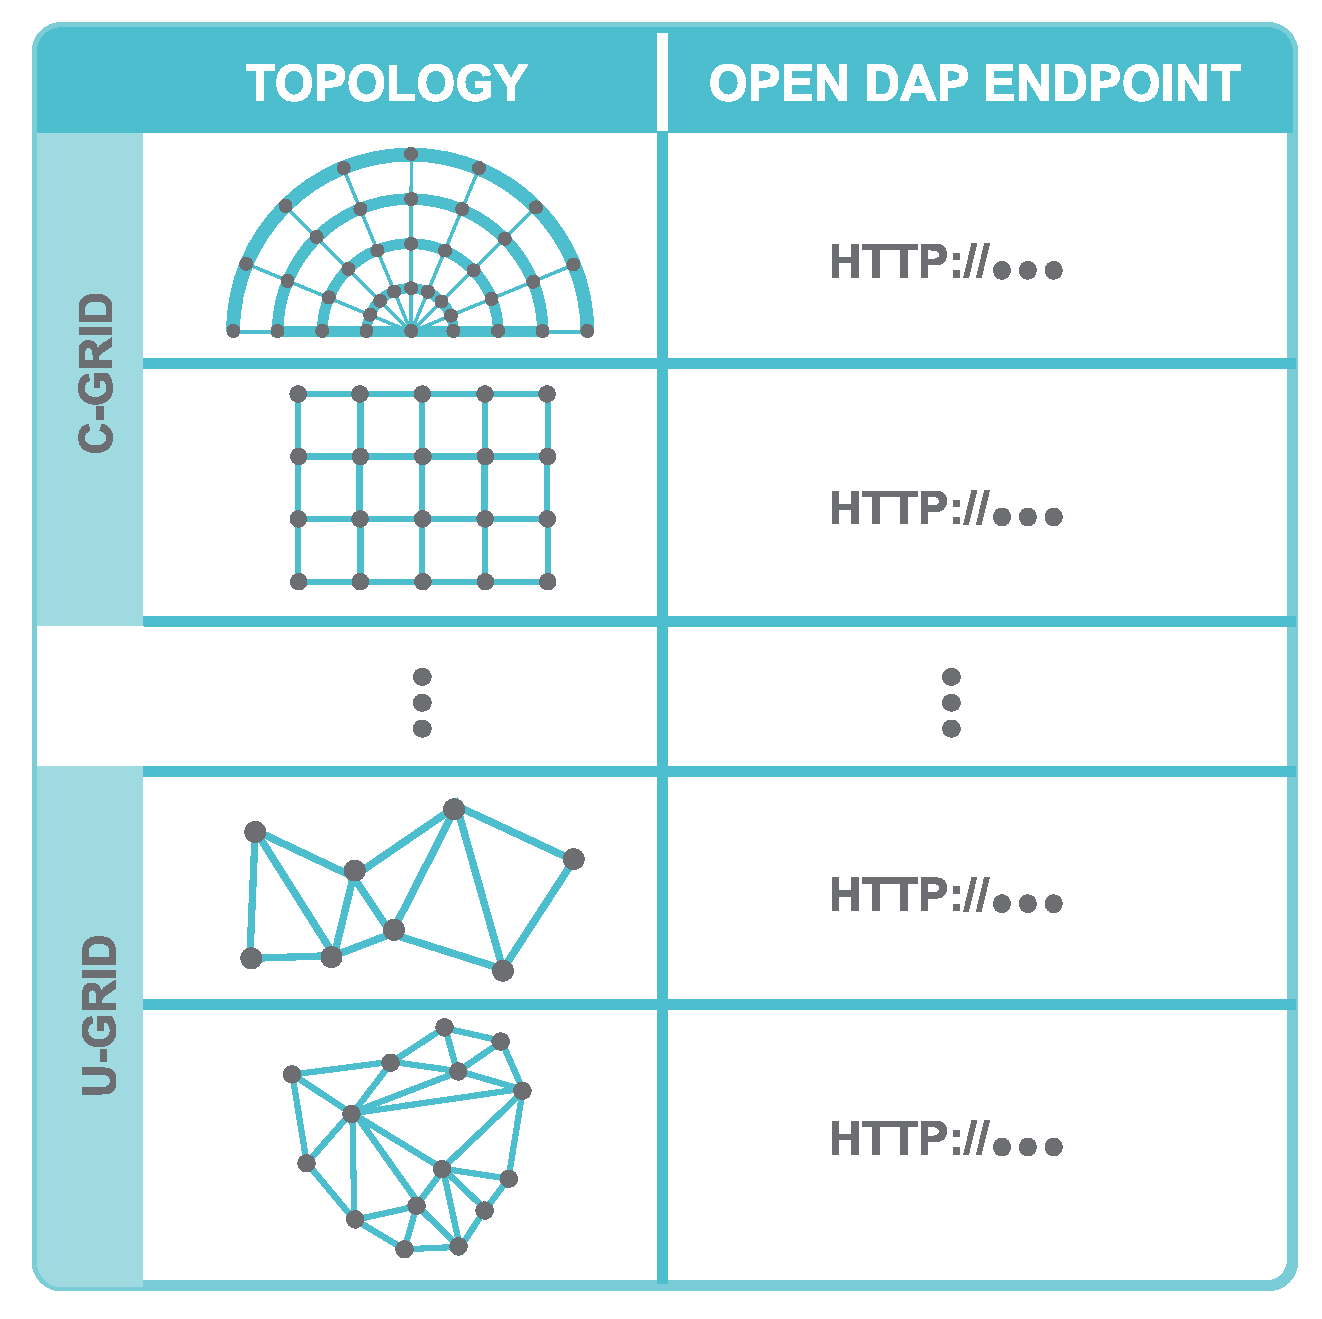
\includegraphics[height=2in]{../figs/sciwms_book_db_topology_endpoint_chart}
%%   \caption{\Sciwms{} topology and endpoint data store.}
%%   \label{fig:sciwms_topology_endpoints}
%% \end{figure}


